%%%%%%%%%%%%%%%%%%%%%%%%%%%%%%%%%%%%%%%%%
% Journal Article
% LaTeX Template
% Version 1.3 (9/9/13)
%
% This template has been downloaded from:
% http://www.LaTeXTemplates.com
%
% Slightly updated by  Marc Uetz
%
% Original author:
% Frits Wenneker (http://www.howtotex.com)
%
% License:
% CC BY-NC-SA 3.0 (http://creativecommons.org/licenses/by-nc-sa/3.0/)
%
%%%%%%%%%%%%%%%%%%%%%%%%%%%%%%%%%%%%%%%%%

%----------------------------------------------------------------------------------------
%	PACKAGES AND OTHER DOCUMENT CONFIGURATIONS
%----------------------------------------------------------------------------------------

\documentclass[twoside]{article}

\usepackage{lipsum} % Package to generate dummy text throughout this template
\usepackage{amsmath,amssymb,amsthm,appendix,graphicx} % Mathematical Symbols, styles, etc

\newtheorem{theorem}{Theorem}[section]
\newtheorem{lemma}[theorem]{Lemma}
\newtheorem{proposition}[theorem]{Proposition}
\newtheorem{corollary}[theorem]{Corollary}
\newtheorem{definition}{Definition}[section]


\usepackage[sc]{mathpazo} % Use the Palatino font
\usepackage[T1]{fontenc} % Use 8-bit encoding that has 256 glyphs
\linespread{1.05} % Line spacing - Palatino needs more space between lines
\usepackage{microtype} % Slightly tweak font spacing for aesthetics

\usepackage[hmarginratio=1:1,top=32mm,columnsep=20pt]{geometry} % Document margins
\usepackage{multicol} % Used for the two-column layout of the document
\usepackage[hang, small,labelfont=bf,up,textfont=it,up]{caption} % Custom captions under/above floats in tables or figures
\usepackage{booktabs} % Horizontal rules in tables
\usepackage{float} % Required for tables and figures in the multi-column environment - they need to be placed in specific locations with the [H] (e.g. \begin{table}[H])
\usepackage{hyperref} % For hyperlinks in the PDF
\usepackage[dutch]{babel}
\usepackage{lettrine} % The lettrine is the first enlarged letter at the beginning of the text
\usepackage{paralist} % Used for the compactitem environment which makes bullet points with less space between them
\usepackage{algorithmicx}
\usepackage[]{algorithm2e}
\usepackage{algpseudocode}
\usepackage{pifont}
\usepackage{abstract} % Allows abstract customization
\renewcommand{\abstractnamefont}{\normalfont\bfseries} % Set the "Abstract" text to bold
\renewcommand{\abstracttextfont}{\normalfont\small\itshape} % Set the abstract itself to small italic text

\usepackage{titlesec} % Allows customization of titles
%\renewcommand\thesection{\Roman{section}} % Roman numerals for the sections
%\renewcommand\thesubsection{\Roman{subsection}} % Roman numerals for subsections
\titleformat{\section}[block]{\large\scshape}{\thesection.}{1em}{} % Change the look of the section titles
\titleformat{\subsection}[block]{\large}{\thesubsection.}{1em}{} % Change the look of the section titles

\usepackage{fancyhdr} % Headers and footers
\pagestyle{fancy} % All pages have headers and footers
\fancyhead{} % Blank out the default header
\fancyfoot{} % Blank out the default footer
\fancyhead[C]{C.H.M.\ van den Bogaard, D.T.R. Ikink, F.\ Seuren, R.\ Monshouwer: \shorttitle} % Custom header text
\fancyfoot[RO,LE]{\thepage} % Custom footer text

%----------------------------------------------------------------------------------------
%	TITLE SECTION
%----------------------------------------------------------------------------------------

\newcommand{\articletitle}{Fast partition refinement, a Python implementation}
\newcommand{\shorttitle}{Python fast partitioning}

\title{\vspace{-15mm}\fontsize{24pt}{10pt}\selectfont\textbf{\articletitle}} % Article title

\author{
\large
\textsc{Christiaan van den Bogaard, Dion Ikink, Fleur Seuren, and Rogier Monshouwer}\thanks{Thanks to our helpful mentor.}\\[2mm] % Your name
\normalsize University of Twente \\ % Your institution
\normalsize \href{mailto:c.h.m.vandenbogaard@student.utwente.nl}{c.h.m.vandenbogaard@student.utwente.nl},
\href{mailto:d.t.r.ikink@student.utwente.nl}{d.t.r.ikink@student.utwente.nl} \\
\normalsize\href{mailto:f.seuren@student.utwente.nl}{f.seuren@student.utwente.nl}, % Your email addresses
\href{mailto:r.monshouwer@student.utwente.nl}{r.monshouwer@student.utwente.nl}
}

\date{\today}

%----------------------------------------------------------------------------------------

\begin{document}

\thispagestyle{empty}
\maketitle % Insert title

%----------------------------------------------------------------------------------------
%	ABSTRACT
%----------------------------------------------------------------------------------------

\begin{abstract}

\noindent \lipsum[1] % Dummy abstract text

\end{abstract}

%----------------------------------------------------------------------------------------
%	ARTICLE CONTENTS
%----------------------------------------------------------------------------------------

\begin{multicols}{2} % Two-column layout throughout the main article text



%------------------------------------------------
\section*{Introduction}
\begin{quote}
\textit{''Gegeven twee eindige graven G en H, bestaat er een isomorfisme tussen G en H?''}
\end{quote}

Het bovenstaande probleem staat bekend als het graaf isomorfisme probleem  (GI), \'e\'en van de meest bestudeerde onderwerpen binnen de discrete wiskunde en theoretische informatica. Hoewel dit probleem voor verschillende klassen van graven is opgelost  en er honderden onderzoeken over zijn gepubliceerd, is er nog altijd geen effici\"ente oplossing gevonden die toepasbaar is op alle mogelijke grafen. Niet voor niets bevindt de complexiteit van dit probleem zich in een geheel nieuwe complexiteitsklasse, tussen de problemen die oplosbaar zijn in polynomiale tijd (P) en de beslisproblemen wiens oplossingen verifieerbaar zijn in polynomiale tijd (NP-complete).

Een van de bestaande technieken die veel gebruikt wordt om het GI probleem op te lossen is ''partition refinement''. In dit artikel wordt het idee achter ''partition refinement'' uitgelegd. Daarnaast wordt er zeer effici\"ente Python implementatie van deze techniek gegeven worden. Dit algoritme, dat gebaseerd is op een door Hopcroft~\cite{MR0403320} bedacht algoritme voor het minimaliseren van DFA's heeft namelijk een complexiteitklasse van $O(m \log_{2} (n)$ met $m= \text{aantal lijnen}$ en $n = \text{aantal punten}$, terwijl een standaard implementatie maar een tijdscomplexiteitsklasse van $O(n^2)$ heeft.

%------------------------------------------------
\section{Theoretische onderbouwing}
In deze sectie wordt de theorie achter zowel ''partition refinement'' als het algoritme van Hopcroft uitgelegd.

\subsection{Partition refinement}
Het idee achter partition refinement is dat een isomorfisme de omgeving (de verzameling buren) van een punt $v$ in stand houdt. Punt $v$ in graaf $G$ heeft dus dezelfde omgeving als zijn afbeelding $\phi(v)$ in H. Hieruit volgt dat de graad van $v$ gelijk is aan de graad van $\phi(v)$. Er kan dus een initi\"ele partitie gemaakt worden op basis van graad. In dit artikel betekent de kleuring van een graaf hetzelfde als de partionering van een graaf. Door een partitie een kleur toe te wijzen kunnen we makkelijke illustreren hoe de graaf wordt verdeeld. 

Omdat alle punten nu een bepaalde kleur hebben kan deze initi\"ele partitie verfijnd worden, namelijk op basis van de kleuromgeving van punt $v$. Deze kleuromgeving is als volgt gedefinieerd:

\begin{definition}
Neem $\alpha$, een partitie van graaf $G$ met $k$ verschillende kleuren en  $\alpha^{c}$ de verzameling punten van $G$ met kleur $c \in \{1,\ldots,k\}$. Twee punten $u,v \in V(G)$ hebben een \textbf{verschillende kleuromgeving} als er een kleur $c \in \{1,\ldots,k\}$ is zodanig dat $|N(u)\cap\alpha^{c}| \neq |N(v)\cap\alpha^{c}|$. Als dit niet geldt hebben de twee punten een \textbf{gelijke kleuromgeving}
\cite{slides_DFA}
\end{definition}


De partitie wordt nu dus verfijnd door elke groep op te splitsen in punten met een verschillende kleuromgeving, waarbij elke nieuwe groep uiteraard weer een nieuwe kleur krijgt. Omdat er weer punten met nieuwe kleuren zijn bijgekomen kan ook deze partitie weer verfijnd worden op basis van kleuromgeving. Dit proces wordt herhaald tot het niet meer mogelijk is om een groep op te splitsen in nieuwe groepen met verschillende kleuromgevingen. Op dat moment bevinden zich in elke groep alleen maar elementen met dezelfde kleuromgeving, er wordt dan gesproken van een stabiele partitie.

Zoals eerder vermeld was behoud een isomorfisme de omgeving van een bepaald punt, een isomorfisme behoudt dus ook de kleuromgeving van een bepaald punt. In twee isomorfe graven bevindt zich dus een gelijke stabiele partitie. Met behulp van zo'n stabiele partitie kan een van deze drie situaties ontstaan.
\begin{enumerate}
\item Er kan een isomorfisme gedefinieerd worden.
\item Er bestaat geen isomorfisme en dat de twee graven niet isomorf zijn.
\item Het kan zijn dat er het nog geen bijectie ontstaat en het dus nog niet zeker is of er een isomorfisme is.
\end{enumerate}

\subsection{Hopcrofts algoritme}
Het nadeel van bovenstaand algoritme is dat, hoewel het een enorme verbetering is ten opzichte van een brute force methode nog steeds een complexiteit van $O(n^2)$ heeft, nog niet heel effici\"ent dus. Daarom is er gezocht naar een snellere implementatie van dit algoritme, zoals het algoritme van Hopcroft. Er wordt dus nog steeds gezocht naar een stabiele partitie $\alpha$ voor graaf $G$ alleen we zoeken deze in een zo minimaal aantal stappen, de ruwste stabiele partitie.

\begin{lemma}
Neem C een kleurgroep in de huidige partitie $\alpha$ en definieer voor alle $i \geq 0$ $D_{i}$ als het aantal punten met precies $i$ buren in $C$. Door elke kleurgroep $C' \neq C$ in de huidige partitie te vervangen door de niet-lege kleurgroepen $C'_{i} := C'\cap D_{i}$ wordt de ruwste stabiele partitie voor graaf $G$ gevonden.
\cite{slides_DFA}
\end{lemma}


De verfijning die hierboven beschreven staat kan ge\"implementeerd worden met een complexiteitsklasse van $O(|E^{-}(C)|)$. Dat komt omdat bij iedere iteratie van het algoritme het niet nodig is om de punten in alle overige kleurklassen te checken.

\begin{lemma}
Stel $C \subseteq V(G)$ wordt tijdens een iteratie gesplitst in $C_{0}, \ldots, C_{k}$. Dan geldt $\forall a \in \{0,\ldots,k\}$: als partitie $\alpha$ stabiel is voor $C$ en voor $C_{b}$ $\forall b \in \{0,\ldots,k\}/\{a\}$, dan is partitie $\alpha$ ook stabiel voor $C_{a}$.
\end{lemma}

\begin{proof}
Stel $\alpha$ is niet stabiel voor $C_{a}$:\\
Dan: $ u,v \in V(G)$ met $u \equiv_{\pi} v$ zodanig dat $u \in C_{a}$ en $v \not \in C_{a}$.\\
Omdat partitie $\alpha$ stabiel was voor $C$ geldt: $u,v \in C$.\\
Omdat $C_{0},\ldots,C_{a},\ldots,C{k}$ een partitie is van $C$ geldt: $\exists b \neq a $ zodanig dat $v \in C_{a}$ en $u \not \in C_{a}$.\\
Dan geldt: $\alpha$ is niet stabiel voor $C_{b}$, een tegenstelling.
\cite{slides_DFA}
\end{proof}


Het is dus niet nodig om de partitie te verfijnen voor alle kleurklassen, waardoor de tijdscomplexiteit stijgt.

In de volgende sectie zal de Python implementatie voor een algoritme beschreven worden en bewezen worden dat deze een complexiteitsklasse van $O(|E^{-}(C)|)$ heeft.
%------------------------------------------------

\section{Implementatie}
Het algoritme staat hieronder in psuedocode, maar we zullen het ook kort even toelichten. We beginnen alle vertices $v_i$ in te delen in een partitie $C_j$ op basis van degree. Vervolgens stoppen wij alle partities in een queue(Q).
Zolang Q niet leeg is, halen wij de eerste color C uit Q. 
Dan kan je partities $ C' $ splitsen in nieuwe partities op basis van hoeveel buren ze in C hebben. Dit doen we door $ \forall V_i \in C $ te bekijken wat hun buren $V'$ zijn. Hoe vaak $V'$ hierin wordt  gezien als buur wordt bijgehouden in een $neighbour\_count$. Zodra je door alle $V'$ bent geitereerd, bekijk alle $C'$ van de vertices $V'$. Zodra er tussen $ \forall{V'} \in C $ er een verschil in $neighbour\_count$ zit, maak je nieuwe partities bijbehorende bij die $neighbour\_count$. Zo wordt bijv $ \forall_{V' \in C'}  [ neighbour\_count(V') = 0] $ een partitie.

\begin{algorithm}[H]
 \KwData{Een graaf $G(V,E)$ }
 \KwResult{Een stabiele partitie $a_{i}$ of G }
initalization \;
 \ForAll{ $v$ $\in$ $V(G)$ }{
	$\alpha(v) := v.degree()$
}
 $queue := [\alpha]$\;
 \While{$queue$ nonempty}{
  $c := dequeue(queue)$\;
  $d\_count := generate\_dcount(c)$\;
  \ForAll{$ color_{i} \in d\_count$}{
   \If{ $d\_count(color_{i}) > 1 $ }{
	$new\_color := x_{1} \in d\_counts(color_{i})$ \;
	\ForAll{ $ x_{i} \in d\_counts(color_{i}) | x_{i} \neq x_{1} $}{
	$c_{i} = x_{i} $ 
	}
   \eIf{$ new\_color \in queue $}{
	$ queue = \{c_{i}\} \cup queue $ \;
  } {
	neem grootste partitie
	$ F := max(\{ c_{i}, new\_color \} ) $ \;
	$ queue = \{ \{ new\_color \} / F \} \cup queue $

}	



  }
 }
}

 \caption{fast partition refinement}
\end{algorithm}
\pagebreak

\begin{algorithm}[H]
 \KwData{Een partitie $C$}
 \KwResult{Een Mapping $ \beta(c') \mapsto \gamma(neighbourcount) \mapsto \{ V_{i} \} $}
Een partitie mapt naar een mapping van een aantal buren, die weer mapt aan een lijst met vertices die dat aantal buren hebben. Zo kunnen wij gemakkelijk splitsen in nieuwe partities \;
 \ForAll{ $v$ $\in$ $C$ }{
\ForAll{ $v'$ $\in$ $N(v)$ }{
	$ neighbour\_count(v') =+ 1 $ \;
	$ colorset = colorset \cup  neighbour.colorclass  $  \;
}	
}


  \ForAll{$ color_{i} \in colorset $}{

	
	\ForAll{ $ v \in color_{i} $ }{
	\eIf{ $ v \in neighbour\_count $} {
	 	$ nbscount := neighbour\_count(v) $ \;
	} {
	$ nbscount := 0 $ \;
	$ d\_count(0) \cup v $ \;
	}
}
$ result(c) \cup d\_count $

	
  }
return result
 
\caption{$ generate\_dcount $}

\end{algorithm}




%------------------------------------------------
\subsection{Bewijs}

We gaan hier bewijzen dat de tijdscomplexiteit van  $ Refine(C) $ $ O(|E(C)|)$ ,  waar $ E(C) $ het aantal lijnen is.

\begin{lemma}
De complexiteit van $Refine(C)$ van een graaf is $O(|E(C)|) $,  waarbij  $ E(C)$ het aantal lijnen incident met vertices in $C$
\end{lemma}

Bewijs:
De operatie $ Refine(C) $ kan gezien worden als $ \forall_{C'} $  $ C' \neq C $ $ Refine(C, C') $. $Refine(C, C') $ itereert langs $ E(C') $  incident met $ C$ . 
Laten we de notatie $ E(C', C) $ het aantal lijnen noemen vanuit $ C' $ naar $ C $
Er geldt dus ook dat $ \forall_{C'}  $  $ C' \neq C $  $ E(C', C) \leqslant E(C) $
Dus de operatie $ Refine(C) $ heeft een complexiteit van $O(|E(C)|$ 



%------------------------------------------------
\section{Berekende resultaten}

De resultaten van de metingen zijn gegeven in Appendix~\ref{AppendixA}.

Om toeval uit te sluiten zijn alle tests tien keer uitgevoerd voor beide algoritmes. De gemeten tijden zijn de gemiddelden van de tien uitgevoerde tests. In de laatste kolom is het verschil in uitvoertijd opgenomen, weergegeven als percentages. Een percentage van $100$\% betekent dat het Fast Refine-algoritme (FR) tweemaal zo snel was als het Refine-algoritme (R) bij het uitvoeren van de test (een verbetering van $100$\% ten opzichte van Refine).

Wat opvalt is dat FR pas bij grote grafen significant sneller is. bigtrees1 bevat vier grafen, elk met 44 vertices. bigtrees3 bevat ook vier grafen, maar elk van deze grafen heeft maar liefst 227 vertices. bigtrees3 heeft dus ruim vijf maal zo veel vertices als bigtrees1. Voor bigtrees1 is FR ongeveer 6\% sneller dan R, terwijl dat percentage voor bigtrees3 vele malen hoger ligt: FR is bijna achttien keer sneller.

De 'threepaths' grafen zijn complexe problemen voor het Color Refinement-algoritme om op te lossen. Ze bevatten lange paden en in elk pad kunnen er maximaal twee vertices van kleur veranderen (zie Figuur~\ref{paths}). Dit heeft tot gevolg dat R zeer veel tijd nodig heeft om tot een stabiele partitie te komen. FR pakt het probleem zoals verwacht veel effici\"enter aan. Voor een van de grotere grafen (threepaths5120) is FR ruim 25 keer sneller.

\begin{figure}[H]
\centering
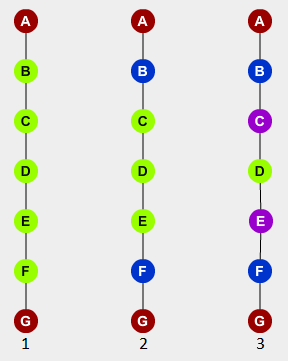
\includegraphics[]{paths.png}
\caption{In graaf 1 is de partitie na de eerste stap van het algoritme gegeven. Graaf 2 is het resultaat van de volgende iteratie. Aangezien vertices B en F nu veranderd zijn, moeten alle vertices daartussen (C, D en E) ook opnieuw bekeken worden. Zoals hier te zien is kan het algoritme per iteratie maar voor twee vertices in een pad de coloring verfijnen. Graaf 3 geeft de stabiele coloring weer. \label{paths}}
\end{figure}


%------------------------------------------------
\section{Conclusie}
Het blijkt dus dat Hopcrofts algoritme een slimme manier is om een graaf te partitioneren. Het grote graaf isomorfisme probleem blijkt een lastige opgave te zijn en color refinement is de veelzijdige hamer in de gereedschapskist om het graaf isomorfisme op te lossen. Het helpt de graaf te onderscheiden in verschillende partities waardoor een bijectie kan ontstaan. John Hopcrofts idee achter DFA minimalisatie bleek een perfecte oplossing om zo snel mogelijk een graaf te partitioneren. Door de grootste partitie niet verder te bezoeken onstaat er een logaritmische partionering waar alleen het zoeken naar de verschillende partities een linear complexiteit heeft. Dit is een hele verbetering ten opzichte van het standaard refine algoritme. Door beide algoritmes te implementeren in python konden we concluderen: 1. Onze implementatie bewijst dat het mogelijk is om Hopcrofts algoritme te implementeren in de tijdscomplexiteitsklasse van orde $O(m\log_{2}(n))$ door te bewijzen dat ``Refine`` in lineaire tijd loopt en een slimme queue regel zodat alleen de kleinste nieuwe partities in de queue komen. 2. Testgrafen laten zien dat FR altijd sneller is dan de eenvoudige versie R. Vooral voor complexe grafen zoals threepaths laat onze implementatie erg goede resultaten zien.

\section{Discussie}
Hoewel onze implementatie al heel erg snel is, hebben we nog een aantal verbetering bedacht die door ons of anderen gebruikt kan worden voor een nog sneller algoritme. De eerste verbetering is een slimmere queue, waardoor het algoritme voor veel grafen in lineaire tijd kan partitioneren. Wij hebben dit gezien bij anderen en wij geloven dat dit ook een echte verbetering voor onze implementatie kan zijn. De tweede verbetering is bedoeld voor het tellen van het aantal automorfismen van een graaf. Dat hebben we in dit artikel niet uitgelegd maar het probleem is nauw verwant aan het graaf isomorfisme probleem. Een automorfisme van een graaf is een isomorfisme op zich zelf. Door de recursieboom van het aantal automorfisme te optimaliseren kunnen we samen met FR een effectief algoritme cre\"eren om het automorfisme probleem op te lossen.\cite{slides_aut}\\
Verder kunnen we uit de berekende data nog niet concluderen dat de tijdscomplexiteitsklasse veranderd is ten opzichte van het standaard algoritme R. Dit kan komen doordat: 
\begin{itemize}
\item Algoritme R is ook erg goed ge\"implementeerd waardoor het in dezelfde tijdscomplexiteitsklasse valt.
\item Algoritme FR is nog niet optimaal waardoor het dezelfde asymptotisch gedrag toont als R.
\item De grafen die getest zijn waren nog niet groot genoeg om een goed onderscheid te kunnen maken tussen de twee algoritmes.
\end{itemize}
Om achter de oorzaak van dit probleem te komen moeten er nog verder onderzoek gedaan worden.


%----------------------------------------------------------------------------------------
%	REFERENCE LIST
%----------------------------------------------------------------------------------------

% Bibliography - this is intentionally simple in this template
\bibliographystyle{plain}
\bibliography{referenties}
\end{multicols}

%----------------------------------------------------------------------------------------

%----------------------------------------------------------------------------------------
%	APPENDICES
%----------------------------------------------------------------------------------------
\newpage
\section{Appendices}
\subsection{Appendix A: Meetresultaten} \label{AppendixA}

\begin{table}[H]
\caption{Resultaten}\label{table:resultaten}
\centering
\begin{tabular}{lrrr}
\toprule
Graaf & Fast Refine (ms) & Refine (ms) & Verschil \\
\midrule
\midrule
bigtrees1 & $56,2$ & $59,4$ & $5,69$\% \\
bigtrees2 & $137,6$ & $255,5$ & $85,68$\% \\
bigtrees3 & $1865,5$ & $33138$ & $1676,36$\% \\
cographs1 & $35,7$ & $70,6$ & $97,76$\% \\
colorref\_largeexample\_4\_1026 & $932,4$ & $2834,1$ & $203,96$\% \\
colorref\_largeexample\_6\_960 & $1925,5$ & $35804$ & $1759,47$\% \\
colorref\_smallexample\_2\_49 & $3,2$ & $5,1$ & $59,38$\% \\
colorref\_smallexample\_4\_7 & $2$ & $2,4$ & $20,00$\% \\
colorref\_smallexample\_4\_16 & $4,5$ & $6,4$ & $42,22$\% \\
colorref\_smallexample\_6\_15 & $9,3$ & $14,1$ & $51,61$\% \\
cubes3 & $8,7$ & $10,1$ & $16,09$\% \\
cubes4 & $39,2$ & $47,3$ & $20,66$\% \\
cubes5 & $124,1$ & $228,1$ & $83,80$\% \\
products72 & $678,8$ & $1262,6$ & $86,00$\% \\
threepaths160 & $4,4$ & $5,7$ & $29,55$\% \\
threepaths320 & $10$ & $10,5$ & $5,00$\% \\
threepaths640 & $20,7$ & $21,5$ & $3,86$\% \\
threepaths1280 & $36,6$ & $39,1$ & $6,83$\% \\
threepaths2560 & $72$ & $88,6$ & $23,06$\% \\
torus24 & $63,8$ & $100,3$ & $57,21$\% \\
torus144 & $57594$ & $176635$ & $206,69$\% \\
trees36 & $39,5$ & $80,4$ & $103,54$\% \\
trees90 & $67,1$ & $159,2$ & $137,26$\% \\
wheeljoin14 & $271,7$ & $410$ & $50,90$\% \\
wheelstar12 & $460,6$ & $902,7$ & $95,98$\% \\
modulesC & $242922$ & $397950$ & $63,82$\% \\

\bottomrule
\end{tabular}
\end{table}

\end{document}
